\tikzset{every picture/.style={line width=0.75pt}} %set default line width to 0.75pt        

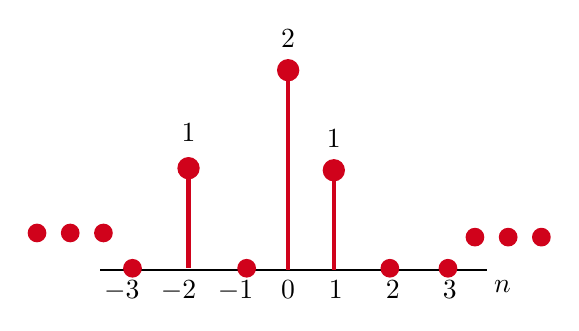
\begin{tikzpicture}[x=0.75pt,y=0.75pt,yscale=-1,xscale=1]
%uncomment if require: \path (0,437); %set diagram left start at 0, and has height of 437

%Straight Lines [id:da6960321259995674] 
\draw    (311.71,160) -- (125.29,160) ;
%Straight Lines [id:da40935280908685534] 
\draw [color={rgb, 255:red, 208; green, 2; blue, 27 }  ,draw opacity=1 ][line width=1.5]    (216,63.58) -- (216,160) ;
\draw [shift={(216,63.58)}, rotate = 90] [color={rgb, 255:red, 208; green, 2; blue, 27 }  ,draw opacity=1 ][fill={rgb, 255:red, 208; green, 2; blue, 27 }  ,fill opacity=1 ][line width=1.5]      (0, 0) circle [x radius= 4.36, y radius= 4.36]   ;
%Straight Lines [id:da27098747867922146] 
\draw [color={rgb, 255:red, 208; green, 2; blue, 27 }  ,draw opacity=1 ][line width=1.5]    (238,111.79) -- (238,160) ;
\draw [shift={(238,111.79)}, rotate = 90] [color={rgb, 255:red, 208; green, 2; blue, 27 }  ,draw opacity=1 ][fill={rgb, 255:red, 208; green, 2; blue, 27 }  ,fill opacity=1 ][line width=1.5]      (0, 0) circle [x radius= 4.36, y radius= 4.36]   ;
%Straight Lines [id:da13999635812051947] 
\draw [color={rgb, 255:red, 208; green, 2; blue, 27 }  ,draw opacity=1 ][line width=1.5]    (168,110.79) -- (168,159) ;
\draw [shift={(168,110.79)}, rotate = 90] [color={rgb, 255:red, 208; green, 2; blue, 27 }  ,draw opacity=1 ][fill={rgb, 255:red, 208; green, 2; blue, 27 }  ,fill opacity=1 ][line width=1.5]      (0, 0) circle [x radius= 4.36, y radius= 4.36]   ;
%Shape: Circle [id:dp7665960437062732] 
\draw  [color={rgb, 255:red, 208; green, 2; blue, 27 }  ,draw opacity=1 ][fill={rgb, 255:red, 208; green, 2; blue, 27 }  ,fill opacity=1 ] (137,159) .. controls (137,156.79) and (138.79,155) .. (141,155) .. controls (143.21,155) and (145,156.79) .. (145,159) .. controls (145,161.21) and (143.21,163) .. (141,163) .. controls (138.79,163) and (137,161.21) .. (137,159) -- cycle ;
%Shape: Circle [id:dp436359616871549] 
\draw  [color={rgb, 255:red, 208; green, 2; blue, 27 }  ,draw opacity=1 ][fill={rgb, 255:red, 208; green, 2; blue, 27 }  ,fill opacity=1 ] (192,159) .. controls (192,156.79) and (193.79,155) .. (196,155) .. controls (198.21,155) and (200,156.79) .. (200,159) .. controls (200,161.21) and (198.21,163) .. (196,163) .. controls (193.79,163) and (192,161.21) .. (192,159) -- cycle ;
%Shape: Circle [id:dp9890944921306494] 
\draw  [color={rgb, 255:red, 208; green, 2; blue, 27 }  ,draw opacity=1 ][fill={rgb, 255:red, 208; green, 2; blue, 27 }  ,fill opacity=1 ] (261,159) .. controls (261,156.79) and (262.79,155) .. (265,155) .. controls (267.21,155) and (269,156.79) .. (269,159) .. controls (269,161.21) and (267.21,163) .. (265,163) .. controls (262.79,163) and (261,161.21) .. (261,159) -- cycle ;
%Shape: Circle [id:dp881688459697376] 
\draw  [color={rgb, 255:red, 208; green, 2; blue, 27 }  ,draw opacity=1 ][fill={rgb, 255:red, 208; green, 2; blue, 27 }  ,fill opacity=1 ] (289,159) .. controls (289,156.79) and (290.79,155) .. (293,155) .. controls (295.21,155) and (297,156.79) .. (297,159) .. controls (297,161.21) and (295.21,163) .. (293,163) .. controls (290.79,163) and (289,161.21) .. (289,159) -- cycle ;
%Shape: Circle [id:dp9509429138475404] 
\draw  [color={rgb, 255:red, 208; green, 2; blue, 27 }  ,draw opacity=1 ][fill={rgb, 255:red, 208; green, 2; blue, 27 }  ,fill opacity=1 ] (123,142) .. controls (123,139.79) and (124.79,138) .. (127,138) .. controls (129.21,138) and (131,139.79) .. (131,142) .. controls (131,144.21) and (129.21,146) .. (127,146) .. controls (124.79,146) and (123,144.21) .. (123,142) -- cycle ;
%Shape: Circle [id:dp9940340579577291] 
\draw  [color={rgb, 255:red, 208; green, 2; blue, 27 }  ,draw opacity=1 ][fill={rgb, 255:red, 208; green, 2; blue, 27 }  ,fill opacity=1 ] (107,142) .. controls (107,139.79) and (108.79,138) .. (111,138) .. controls (113.21,138) and (115,139.79) .. (115,142) .. controls (115,144.21) and (113.21,146) .. (111,146) .. controls (108.79,146) and (107,144.21) .. (107,142) -- cycle ;
%Shape: Circle [id:dp3557855538501913] 
\draw  [color={rgb, 255:red, 208; green, 2; blue, 27 }  ,draw opacity=1 ][fill={rgb, 255:red, 208; green, 2; blue, 27 }  ,fill opacity=1 ] (91,142) .. controls (91,139.79) and (92.79,138) .. (95,138) .. controls (97.21,138) and (99,139.79) .. (99,142) .. controls (99,144.21) and (97.21,146) .. (95,146) .. controls (92.79,146) and (91,144.21) .. (91,142) -- cycle ;
%Shape: Circle [id:dp49757143963020933] 
\draw  [color={rgb, 255:red, 208; green, 2; blue, 27 }  ,draw opacity=1 ][fill={rgb, 255:red, 208; green, 2; blue, 27 }  ,fill opacity=1 ] (334,144) .. controls (334,141.79) and (335.79,140) .. (338,140) .. controls (340.21,140) and (342,141.79) .. (342,144) .. controls (342,146.21) and (340.21,148) .. (338,148) .. controls (335.79,148) and (334,146.21) .. (334,144) -- cycle ;
%Shape: Circle [id:dp1192153550884405] 
\draw  [color={rgb, 255:red, 208; green, 2; blue, 27 }  ,draw opacity=1 ][fill={rgb, 255:red, 208; green, 2; blue, 27 }  ,fill opacity=1 ] (318,144) .. controls (318,141.79) and (319.79,140) .. (322,140) .. controls (324.21,140) and (326,141.79) .. (326,144) .. controls (326,146.21) and (324.21,148) .. (322,148) .. controls (319.79,148) and (318,146.21) .. (318,144) -- cycle ;
%Shape: Circle [id:dp8865578210167575] 
\draw  [color={rgb, 255:red, 208; green, 2; blue, 27 }  ,draw opacity=1 ][fill={rgb, 255:red, 208; green, 2; blue, 27 }  ,fill opacity=1 ] (302,144) .. controls (302,141.79) and (303.79,140) .. (306,140) .. controls (308.21,140) and (310,141.79) .. (310,144) .. controls (310,146.21) and (308.21,148) .. (306,148) .. controls (303.79,148) and (302,146.21) .. (302,144) -- cycle ;

% Text Node
\draw (313.71,163.4) node [anchor=north west][inner sep=0.75pt]    {$n$};
% Text Node
\draw (216,163.4) node [anchor=north] [inner sep=0.75pt]    {$0$};
% Text Node
\draw (190.66,163.4) node [anchor=north] [inner sep=0.75pt]    {$-1$};
% Text Node
\draw (163.24,163.4) node [anchor=north] [inner sep=0.75pt]    {$-2$};
% Text Node
\draw (135.82,163.4) node [anchor=north] [inner sep=0.75pt]    {$-3$};
% Text Node
\draw (239,163.4) node [anchor=north] [inner sep=0.75pt]    {$1$};
% Text Node
\draw (266.42,163.4) node [anchor=north] [inner sep=0.75pt]    {$2$};
% Text Node
\draw (293.84,163.4) node [anchor=north] [inner sep=0.75pt]    {$3$};
% Text Node
\draw (168,99.39) node [anchor=south] [inner sep=0.75pt]    {$1$};
% Text Node
\draw (238,102.39) node [anchor=south] [inner sep=0.75pt]    {$1$};
% Text Node
\draw (216,54.18) node [anchor=south] [inner sep=0.75pt]    {$2$};


\end{tikzpicture}
